\subsection{\Ac{cadx}: Feature detection} \label{subsec:chp3:img-clas:CADX-fea-dec}

Discriminative features which can be used to recognize \ac{cap} from healthy tissue have to be first detected.
This processing is known in computer vision as feature extraction. 
However, feature extraction is also the name given in pattern recognition to some types of dimension reduction methods which will be presented next.
In order to avoid confusion between these two aspects, in this survey, the procedure ``detecting'' or ``extracting'' features from images and signals will be defined as feature detection.
This section will summarize the different strategies employed for this task.
The features used in the studies are summarized in Table.~\ref{tab:feat}.  

\subsubsection{Image-based features}\label{subsubsec:chp3:img-clas:CADX-fea-dec:Img-fea}

This section will focus on image-based features detection.
Two main strategies to detect features have been identified and used for the purpose of our classification: (i) voxel-wise detection and (ii) region-wise detection.

\paragraph{Voxel-wise detection:}
This strategy refers to the fact that a feature is extracted at each voxel location.
\ac{cap} as previously discussed (see Tab.~\ref{tab:modmri}) can be discerned due to \ac{si} changes.
Hence, intensity-based features are one of the most common features used to build the feature vector which has to be classified~\cite{Ampeliotis2007,Ampeliotis2008,Artan2009,Artan2010,Chan2003,Langer2009,Liu2009,Niaf2011,Niaf2012,Viswanath2008a,Viswanath2011}.
This type of feature consists simply of the \ac{si} of each voxel of the different \ac{mri} modalities.

Edge based features have also been used to detect \ac{si} changes.
Each feature is computed by convolving the original image with an edge operator.
Three of these operators are used: (i) Prewitt operator \cite{Prewitt1970}, (ii) Sobel operator \cite{Sobel1970} and (iii) Kirsch operator \cite{Kirsch1971}.
Results obtained with these operators vary, due to their different kernels.
These features are commonly incorporated in the feature vector for further classification in the \ac{cad} systems reviewed \cite{Niaf2011,Niaf2012,Tiwari2009a,Tiwari2010,Tiwari2013,Viswanath2008,Viswanath2011}.

\begin{figure}
	\hspace*{\fill}
		\subfigure[$\theta=0^{\circ}$.]{\label{subfig:gab1} 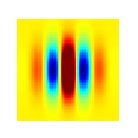
\includegraphics[width=0.2\linewidth]{3_review/figures/feature-detection/gabor/gabor_1.eps}} \hfill
		\subfigure[$\theta=60^{\circ}$.]{\label{subfig:gab2} 
\includegraphics[width=0.2\linewidth]{3_review/figures/feature-detection/gabor/gabor_2.eps}} \hfill
		\subfigure[$\theta=120^{\circ}$.]{\label{subfig:gab3} 
\includegraphics[width=0.2\linewidth]{3_review/figures/feature-detection/gabor/gabor_3.eps}} \hfill
		\subfigure[$\theta=180^{\circ}$.]{\label{subfig:gab4} 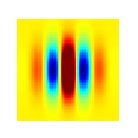
\includegraphics[width=0.2\linewidth]{3_review/figures/feature-detection/gabor/gabor_4.eps}}
	\hspace*{\fill}
	\caption[Illustration of four different Gabor filters.]{Illustration of four different Gabor filters varying their orientations $\theta$.}
	\label{fig:gabor}
\end{figure}

Gabor filters \cite{Gabor1946,Daugman1985} offer another approach to extract information related to edges and texture and were integrated in three different \ac{cad} for \ac{cap} \cite{Viswanath2008a,Viswanath2012,Tiwari2012}.
A Gabor filter is defined by the modulation of a Gaussian function with a sinusoid which can be further rotated.
Hence, a Gabor filter $g$ can be formalized as:
\begin{equation}
	g(x,y;\theta,\psi,\sigma,\gamma) = \exp \left( - \frac{x'^{2}+ \gamma^{2}y'^{2}}{2 \sigma^{2}} \right) \cos \left( 2 \pi \frac{x'}{\lambda} + \phi \right) \ ,
\end{equation}

\noindent with 

\begin{eqnarray}
	x' & = & s\left( x \cos \theta + y \sin \theta \right) \ , \nonumber \\
	y' & = & s \left( - x \sin \theta + y \cos \theta \right) \ , \nonumber
\end{eqnarray}

\noindent where $\lambda$ is the wavelength of the sinusoidal factor, $\theta$ represents the orientation of the Gabor filter, $\psi$ is the phase offset, $\sigma$ is the standard deviation of the Gaussian envelope, $\gamma$ is the spatial aspect ratio and $s$ is the scale factor.
To perform Gabor analysis to extract features for a classification scheme, a bank of Gabor filters is usually created with different angles, scale and dilatations (see Fig.~\ref{fig:gabor}) and then convolved with the image. 

Texture-based features provide other characteristics discerning \ac{cap} from healthy tissue.
The most common texture analysis for image classification are co-occurrence matrices with their related statistics which were proposed in \cite{Haralick1973} and areB commonly used in \ac{cad} systems \cite{Antic2013,Niaf2011,Niaf2012,Tiwari2009a,Tiwari2010,Tiwari2013,Viswanath2008,Viswanath2008a,Viswanath2011,Viswanath2012}.
At each voxel, a neighbourhood is defined around this center and a gray-level co-occurrence matrix is built by selecting a pair of voxels based on a defined distance and angle.
Then, using this co-occurrence matrix, a set of features can be computed based on the statistics describing the texture around each voxel.
Computation of these features is presented in Tab.~\ref{tab:glcm}.

\begin{table}
	\caption{The fourteen statistical features for texture analysis commonly computed from the gray level co-occurrence matrix $p$ as presented by \cite{Haralick1973}.}
	\small
	\renewcommand{\arraystretch}{1.5}
	\begin{tabular}{p{.4\linewidth} p{.6\linewidth}}
		\hline %\\ [-1.5ex]
		\textbf{Statistical features} & \textbf{Formula} \\ \\ [-3ex]
		\hline \\ [-1.5ex]
		Angular second moment & $\sum_i \sum_j p(i,j)^2 \ .$  \\
		Contrast & $\sum_{n=0}^{N_g - 1} n^2 \{ \sum_{i=1}^{N_g - 1} \sum_{j=1}^{N_g - 1} p(i,j) \} \ , | i-j |=n \ . $ \\
		Correlation & $\frac{\sum_i \sum_j (ij) p(i,j) - \mu_x \mu_y}{\sigma_x \sigma_y} \ . $ \\
		Variance & $\sum_i \sum_j (i - \mu)^2 p(i,j) \ . $ \\
		Inverse difference moment & $\sum_i \sum_j \frac{1}{1+(i - \mu)^2} p(i,j) \ . $ \\
		Sum average & $\sum_{i=2}^{2N_g} i p_{x+y}(i) \ . $ \\
		Sum variance & $\sum_{i=2}^{2N_g} (i-f_s)^2 p_{x+y}(i) \ . $ \\
		Sum entropy & $ - \sum_{i=2}^{2N_g} p_{x+y}(i) \log p_{x+y}(i) \ . $ \\
		Entropy & $ - \sum_i \sum_j p(i,j) \log p(i,j) \ .$ \\
		Difference variance & $\sum_{i=0}^{N_g-1} i^2 p_{x-y}(i) \ . $ \\
		Difference entropy & $ - \sum_{i=0}^{N_g-1} p_{x-y}(i) \log p_{x-y}(i) \ . $ \\
		Info. measure of corr. 1 & $\frac{S(X;Y)-S_1(X;Y)}{\max(S(X),S(Y))} \ . $ \\
		Info. measure of corr. 2 & $\sqrt{\left( 1 - \exp \left[ -2( H_2(X;Y) - H(X;Y) ) \right] \right)} \ . $ \\
		Max. corr. coeff. & $ \sqrt{\lambda_2} \ , \text{of } Q(i,j) = \sum_k \frac{p(i,k)p(j,k)}{p_x(i)p_y(k)} \ . $ \\
		\\ [-3ex] \hline
	\end{tabular}
	\label{tab:glcm}
\end{table}

Fractal analysis and more precisely a local estimation of the fractal dimension \cite{Benassi1998} describing the texture roughness at a specific location was used in \cite{Lopes2011}.
A wavelet-based method in a multi-resolution framework was used to estimate the fractal dimension.
Cancerous tissue were characterized to have a higher fractal dimension than healthy tissue.

Chan \textit{et al.}~\cite{Chan2003} described the texture using the frequency signature via the \acf{dct} \cite{Ahmed1974}) defining a neighbourhood of $7 \times 7$ pixels for each of the modalities that they used.
The \ac{dct} allows to decompose a portion of image into a coefficients space where few of these coefficients encoded the visually significant information.
The \ac{dct} coefficients are computed such as:

\begin{equation}
	C_{k_1,k_2} = \sum_{m=0}^{M-1} \sum_{n=0}^{N-1} p_{m,n} \cos \left[ \frac{\pi}{M} \left( m + \frac{1}{2} \right) k_1 \right] \cos \left[ \frac{\pi}{N} \left( n + \frac{1}{2} \right) k_2 \right] \ ,
\end{equation}

\noindent where $C_{k_1,k_2}$ is the \ac{dct} coefficient at the position $k_1,k_2$, $M$ and $N$ are the dimension of the neighbourhood and $p_m,n$ is the pixel \ac{si} at the position $p_{m,n}$.

Viswanath \textit{et al.}~\cite{Viswanath2012} projected \ac{t2w} images into the wavelet space, using Haar wavelet, and used the coefficients obtained from the decomposition as features.
%The wavelet family used for the decomposition was the Haar wavelet.

Finally Litjens \textit{et al.} in \cite{Litjens2011} computed the texture map based on \ac{t2w} images using a Gaussian filer bank.
%% Euclidean distance from each voxel to the prostate center as well as the individual distance in the three directions $x$, $y$ and $z$. \cite{Chan2003} embedded the same information but this time using cylindrical coordinate $r$, $\theta$ and $z$ corresponding to the radius, azimuth and elevation respectively.




\paragraph{Region-wise detection:}

Unlike the previous section, another strategy is to study an entire region and extract characteristic features corresponding to this region.
The most common approach reviewed can be classified as statical methods.
First a feature map is computed for the whole image instaed of using single voxels.
Then, \acp{roi} are defined and statistics are extracted from each of these regions.
The most widely used statistics is based on percentiles and is widely used \cite{Antic2013,Litjens2011,Litjens2012,Peng2013,Tiwari2009a,Tiwari2010,Tiwari2013,Viswanath2008,Viswanath2008a,Viswanath2011,Viswanath2012,Vos2008,Vos2008a,Vos2010,Vos2012}.
The percentile used is usually manually determined observing the distribution and corresponds to the best discriminant value differentiating malignant and healthy tissue.

%%%%%%%%%%%%%%%%%%%%%%%%%%%%%%%%%%%%%%%%%%%%%%%%%%%%%%%%% UUUUUUPPPPPPPP TO HERE %%%%%%%%%%%%%%%%%%%%%%%%%%%%%%%%%%%%%%%%%%%%%%%%%%%%%%%%%%%%%%%%%%%%%


%% In addition, statistic-moments such as mean, standard deviation, kurtosis and skewness are also used \cite{Ampeliotis2007,Ampeliotis2008,Antic2013,Niaf2011,Niaf2012,Peng2013}).

%% Another subset of features are anatomic which were also used by \cite{Litjens2012} and \cite{Matulewicz2013}. \cite{Litjens2012} computed the volume, compactness and sphericity related to the region to integrate it in their feature vector to later classify. \cite{Matulewicz2013} introduced four features corresponding to the percentage of tissue belonging to the regions\ac{pz}, \ac{cg}, periurethral region or outside prostate region for the considered \ac{roi}.

%% In contrast to anatomical are histogram-based features. For instance, \cite{Liu2013} introduced four different types of histogram-based features. The first type corresponds to the histogram of the \ac{si} of the image. The second type is the \acf{hog} \cite{Dalal2005}). \Ac{hog} descriptor describes the local shape of the object of interest by using gradient directions distribution. This descriptor is extracted mainly in three steps. First the gradient image and its corresponding magnitude and direction are computed. Then, the \ac{roi} is divided into cells and an oriented-based histogram is generated for each cell. At each pixel location, the orientation of the gradient will vote for a bin of the histogram and this vote is weighted by the magnitude of the same gradient. Finally, The cells are grouped into block and each block is normalized. The third histogram-based type used by \cite{Liu2013} was shape context \cite{Belongie2002}). The shape context is also a way to describe the shape of an object of interest. First, a set of points defining edges have to be detected and for each point of each edge, a log-polar-based histogram is computed using the relative points distribution. The last set of histogram-based feature extracted is based on the framework of \cite{Zhao2012} which is using the Fourier transform of the histogram created via \acf{lbp} \cite{Ojala1996}). \Ac{lbp} is generated by comparing the value of the central pixel with its 8-connected neighbours. Then, in the \ac{roi}, the histogram of the \ac{lbp} distribution is computed. The \acf{dft} of the \ac{lbp} histogram is ised to make the feature invariant to rotation.

%% The last group of region-based feature is based on fractal analysis. The features proposed are based on estimating the fractal dimension which is a statistical index representing the complexity of what is analysed. \cite{Lv2009} proposed two features based on fractal dimension: (i) texture fractal dimension and (ii) histogram fractal dimension. The first feature is based on estimating the fractal dimension on the \ac{si} of each image. Hence, this feature is a statistical characteristic of the image roughness. The second fractal dimension is estimated in the \ac{pdf} of each image and is characteristic of the complexity of the \ac{pdf}. \cite{Lopes2011} proposed a 3D version to estimate the fractal dimension of a volume using wavelet decomposition.


%% \subsubsection{\ac{dce}-based features}\label{subsubsec:fddce}

%% \ac{dce}-\ac{mri} is more commonly based on a \ac{si} analysis over time as presented in Sect.~\ref{subsubsec:mrimrsi}. The parameters extracted used in \ac{cad} system during the \ac{dce}-\ac{mri} analysis are presented

%% \begin{table*}
%% 	\caption{Parameters used as features for a \ac{dce} semi-quantitative analysis in \ac{cad} systems.}
%% 	\footnotesize
%% 	%\renewcommand{\arraystretch}{1.5}
%% 	\begin{tabular}{p{.35\linewidth} p{.60\linewidth}}
%% 		\hline \\ [-1.5ex]
%% 		\textbf{Semi-quantitative features} & \textbf{Explanations} \\ \\ [-1.5ex]
%% 		\hline \\ [-1.5ex]
%% 		\textit{Amplitude features:} & \\ \\ [-1.5ex]
%% 		\quad $S_0$ & Amplitude at the onset of the enhancement \\
%% 		\quad $S_{\max}$ & Amplitude corresponding to $95\%$ of the maximum amplitude \\
%% 		\quad $S_{p}$ & Amplitude corresponding to the maximum amplitude \\
%% 		\quad $S_f$ & Amplitude at the final time point \\ \\ [-1.5ex]
%% 		\textit{Time features:} & \\ \\ [-1.5ex]
%% 		\quad $t_0$ & Time at the onset of the enhancement \\
%% 		\quad $t_{\max}$ & Time corresponding to $95\%$ of the maximum amplitude \\
%% 		\quad $t_{p}$ & Time corresponding to the maximum amplitude \\
%% 		\quad $t_{f}$ & Final time \\
%% 		\quad $t_{tp}$ & Time to peak which is the time from $t_0$ to $t_p$ \\ \\ [-1.5ex]
%% 		\textit{Derivatives and integral features:} & \\ \\ [-1.5ex]
%% 		\quad $WI$ & Wash-in rate corresponding to the signal slope from $t_0$ to $t_m$ or $t_p$ \\
%% 		\quad $WO$ & Wash-out rate corresponding to the signal slope from $t_m$ or $t_p$ to $t_p$ \\
%% 		\quad $IAUC$ & Initial area under the curve which is the area between $t_0$ to $t_{f}$ \\ \\ [-1.5ex]
%% 		\hline
%% 	\end{tabular}
%% 	\label{tab:semiqua}
%% \end{table*}


%% \setenumerate{listparindent=\parindent,itemsep=10px}
%% \setlist{noitemsep}
%% \begin{enumerate}[leftmargin=*]

%% \item[$-$] \textbf{\textit{Whole-spectra approach:}} Some studies are using the whole \ac{dce} time series as feature vector such as \cite{Ampeliotis2007,Ampeliotis2008}, \cite{Tiwari2012} and \cite{Viswanath2008a,Viswanath2008}. In some cases, the high-dimensional feature space is reduced using dimension reduction methods as it will be presented in the next section (see Sect.~\ref{subsec:featureselectionextraction}).

%% \begin{figure}
%% 	\centering
%% 	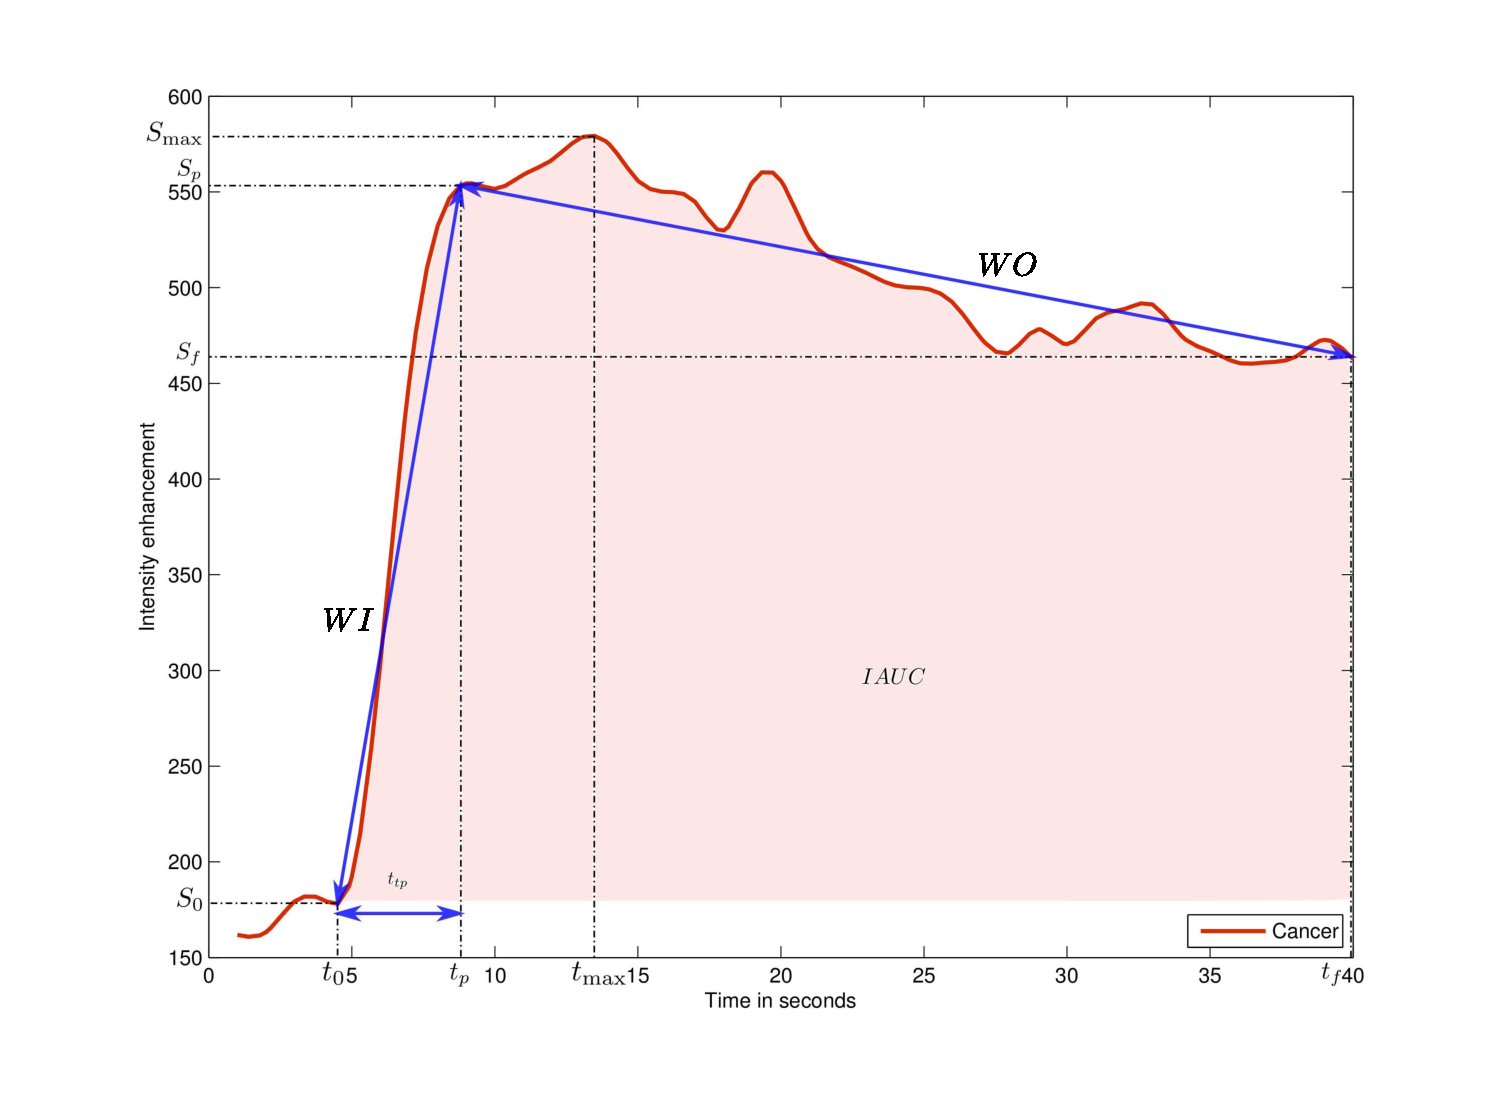
\includegraphics[width=.8\linewidth]{04_data_classification/06_feature_detection/figures/dce/dce_cancer_parameters.eps}
%% 	\caption{Graphical representation of the different semi-quantitative features used for \ac{dce}-\ac{mri} analysis.}
%% 	\label{fig:dceparam}
%% \end{figure}

%% \item[$-$] \textbf{\textit{Semi-quantitative approach:}} Semi-quantitative approaches are based on modelling mathematically the \ac{dce} time series. The parameters modelling the signal are commonly used mainly due to the simplicity of their computation. Parameters included in semi-quantitative analysis are summarized in Tab.~\ref{tab:semiqua} and also graphically depicted in Fig.~\ref{fig:dceparam}. A set of time features corresponding to specific amplitude level (start, maximum and end) are extracted. Then, derivative and integral features are also considered as discriminative and are commonly computed.

%% \item[$-$] \textbf{\textit{Quantitative approach:}} As presented in Sect.~\ref{subsubsec:mrimrsi}, quantitative approaches correspond to mathematical-pharmacokinetic models based on physiological exchanges. Four different models have been used in \ac{cad} systems. 

%% The most common model reviewed was the \textit{Brix model} \cite{Artan2009,Artan2010,Sung2011,Liu2009,Ozer2009,Ozer2010}). This model is formalized such as:
%% \begin{equation}
%% 	\frac{S(t)}{S(0)} = 1 + A k_{ep} \left( \frac{\exp( -k_{ep} t ) - \exp( -k_{el} t )}{k_{el} - k_{ep}} \right) \ ,
%% 	\label{eq:brixmod}
%% \end{equation}

%% \noindent where $S(\cdot)$ is the \ac{dce} signal, $A$ is the parameter simulating the tissue properties, $k_{el}$ is the parameter related to the first-order elimination from the plasma compartment and $k_{ep}$ is the parameter of the transvascular permeability and the parameters $k_{ep}$, $k_{el}$ and $A$ are computed from the \ac{mri} data and used as features.

%% Thus, the parameters $k_{ep}$, $k_{el}$ and $A$ are computed and used as features.

%% The Tofts model \cite{Tofts1997}) was used by \cite{Langer2009,Giannini2013,Niaf2011,Niaf2012,Mazzetti2011}. The \ac{dce} signal relative to the concentration is modelled as:
%% \begin{equation}
%% 	C_t(t) = v_p C_p(t) + K_{trans} \int_{0}^{t} C_p(\tau) \exp( -k_{ep}(t-\tau) ) \ d\tau \ ,
%% 	\label{eq:tofts} 
%% \end{equation}

%% \noindent where $C_t(\cdot)$ is the concentration of the medium, $C_p(\cdot)$ is the \ac{aif} which have to be estimated independently, $K_{trans}$ is the parameter related to the diffuse transport of media across the capillary endothelium, $k_{ep}$ is the parameter related to the exchanges back into the vascular space and $v_e$ is the extravascular-extracellular space fraction defined such that $v_e = 1 - v_p$. Thus, the parameters $K_{trans}$, $k_{ep}$ and $v_e$ are computed and used as features in this model.

%% \cite{Mazzetti2011} and \cite{Giannini2013} used the Weibull function empirically formalized as:
%% \begin{equation}
%% 	S(t) = A t \exp( -t^{B} ) \ ,
%% 	\label{eq:weibull}
%% \end{equation}

%% \noindent where $A$ and $B$ are the two parameters which have to be inferred.

%% They also used another empirical model which is based on the West-like function and named the phenomenological universalities model \cite{Castorina2006}) formalized as:
%% \begin{equation}
%% 	S(t) = \exp \left[ r t + \frac{1}{\beta} a_0 - r \left( \exp( \beta t ) - 1 \right) \right] \ ,
%% 	\label{eq:pun}
%% \end{equation}

%% \noindent where the parameters $\beta$, $a_0$ and $r$ are inferred.

%% For all these models, the parameters are inferred using an optimization curve fitting approach.

%% \end{enumerate}

%% \subsubsection{\ac{mrsi}-based features}

%% \setenumerate{listparindent=\parindent,itemsep=10px}
%% \setlist{noitemsep}
%% \begin{enumerate}[leftmargin=*]

%% \item[$-$] \textbf{\textit{Whole spectra approach:}} As in the case of \ac{dce} analysis, one common approach is to incorporate the whole \ac{mrsi} spectra in the feature vector for classification \cite{Kelm2007,Parfait2012,Tiwari2007,Tiwari2009,Tiwari2013,Tiwari2009a,Tiwari2010,Viswanath2008a,Matulewicz2013}). Sometimes post-processing involving dimension reduction methods is performed to reduce the complexity during the classification as it will be presented in Sect.~\ref{subsec:featureselectionextraction}.

%% \item[$-$] \textbf{\textit{Quantification approach:}} We can reiterate that in \ac{mrsi} only few biological markers (cf., choline, creatine and citrate metabolites mainly) are known to be useful to discriminate \ac{cap} and healthy tissue. Then, concentrations of these metabolites can be considered as a feature used for classification. In order to perform this quantification, four different approaches have been used. The QUEST \cite{Ratiney2005}), AMARES \cite{Vanhamme1997}) and VARPRO \cite{Coleman1993}) models were used by \cite{Kelm2007}. They are all time-domain quantification methods varying by the type of pre-knowledge embedded and the optimization approaches used to solve the quantification problem. Unlike the time-domain quantification approaches, \cite{Parfait2012} used the LcModel approach \cite{Provencher1993}) which solves the optimization problem in the frequency domain.

%% Once the different concentrations are computed, \cite{Kelm2007} calculated the relative concentrations (Eq. \eqref{eq:ratio1} and \eqref{eq:ratio2}) and used them as features. However, \cite{Parfait2012} used each metabolite concentrations individually.

%% \begin{eqnarray}
%% 	R_1 & = & \frac{ [ \text{Cho} ] + [ \text{Cr} ]}{[ \text{Cit} ]} \ . \label{eq:ratio1} \\
%% 	R_2 & = & \frac{[ \text{Cit} ]}{[\text{Cho}]+[\text{Cr}]+[\text{Cit}]} \ , \label{eq:ratio2}
%% \end{eqnarray}

%% \noindent where $\text{Cit}$, $\text{Cho}$ and $\text{Cr}$ are the concentration of citrate, choline and creatine respectively.

%% \item[$-$] \textbf{\textit{Wavelet decomposition approach:}} \cite{Tiwari2012} performed a wavelet packet decomposition \cite{Coifman1992}) with the Haar wavelet basis function and used the coefficients of this decomposition as features for further classification.

%% \end{enumerate}
